



\documentclass[]{standalone}
\usepackage{tikz}


\begin{document}

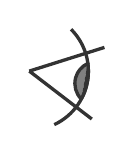
\begin{tikzpicture}[black!80, very thick]

%eye
\pgfmathsetmacro{\eyeSize}{1}
\pgfmathsetmacro{\ex}{0}
\pgfmathsetmacro{\ey}{1}
\pgfmathsetmacro{\eRot}{-10}
\pgfmathsetmacro{\eAp}{-55}
\draw[rotate around={\eRot:(\ex,\ey)}] (\ex,\ey) -- ++(-.5*\eAp:\eyeSize)
     (\ex,\ey) -- ++(.5*\eAp:\eyeSize);
\draw (\ex,\ey) ++(\eRot+\eAp:.75*\eyeSize) arc (\eRot+\eAp:\eRot-\eAp:.75*\eyeSize);

% IRIS
\draw[fill=gray] (\ex,\ey) ++(\eRot+\eAp/3:.75*\eyeSize) % start point
  arc (\eRot+180-\eAp:\eRot+180+\eAp:.28*\eyeSize);

%PUPIL, a filled arc 
\draw[fill=black!80] (\ex,\ey) ++(\eRot+\eAp/3:.75*\eyeSize) % start point
  arc (\eRot+\eAp/3:\eRot-\eAp/3:.75*\eyeSize);

\end{tikzpicture}


\end{document}